\documentclass[a4paper,12pt]{article}

\usepackage[english]{babel}
\usepackage[utf8x]{inputenc}
\usepackage{cite}
\usepackage{hyperref}
\renewcommand{\baselinestretch}{1.2}
\usepackage{indentfirst}
\usepackage{graphicx}
\usepackage{caption}
\usepackage{amsmath}
\usepackage{subcaption}

\usepackage{xcolor}
\usepackage{listings}
\lstset{basicstyle=\ttfamily,
  showstringspaces=false,
  commentstyle=\color{red},
  keywordstyle=\color{blue}
}
        % Set your language (you can change the language for each code-block optionally)
%\usepackage[top=1in,bottom=1in]{geometry}

\begin{document}
\begin{titlepage}
	\centering
	
\includegraphics[width=0.8\textwidth]{logo.eps}\par\vspace{1cm}
	{\scshape\LARGE Vrije Universiteit Brussel\par}
	\vspace{1cm}
	{\scshape\Large Open Information Systems 2017 - 2018\par}
	\vspace{1.5cm}
	{\huge\bfseries Final report - Group 8\par}
	\vspace{2cm}
	{\Large\itshape ROMAIN Maximilien - 0543411\\ (maxromai@ulb.ac.be)\\ ROJAS Felipe - 0542569\\ (felipe.rojas@vub.be)\\PERALE Thomas - 0546990\\ (thomas.perale@vub.be)\\ LEHAL Sherik - 0543118\\ (sherik.lehal@vub.be)\par}
	\vfill

% Bottom of the page
	{\large \today\par}
\end{titlepage}

\newpage


\section{Teamwork}
How did you divide and manage the workload inside your team
We tried to divide the workload equaly for everyone and doing a lot of teamwork to satisfy the requirements of the project also with a lot of communication through Facebook
\section{ER Diagram}
2. Motivate the design behind your conceptual schema
The main objective of the project was to create an online bookstore, where the users can buy and rate ebooks from the database which has sorted the books according to their categories.
All ebooks are identified by their ISBN number. The books also have other attributes such as Year, Title, Publisher which is a different class linked to the main ebook class by "isPublishedby" relation. The ebook class also has a relation to the Category class, which allows users to search different books from different categories. It is also possible to have subcategories inside another category. The author class contains the name, ID of the authors, linked to the ebook class. This further adds more to detail the ebooks.
The user class contains various attribues such as the user ID, name, Payment method etc. This class is linked to the ebook and Purchased class. The purchase class exists to keep a history of all purchases made from the database. The user class also has an attribute, a role class. It specifies wheather the user is an admin, or a normal user. An admin is able to manage all the data. 
The rating class is linked to the ebook class and contains all the rating given to books by the users, after they havepurchased the book.
In short, this allows us to create a system, where the users can login and purchase a book. The user can also check history of their purchases. After purchasing, the user can then rate the book to review it.

\section{Ontologies}
3. Motivate the design your ontologies? 
As our application was relatively straightforward, essentially allowing only ebook purchases, the ontology was also straightforward in seeking to focus on the main elements of our application: its buyers and ebooks. As a result, our ontology has mainly focused on developing interactions between users and ebooks. It can be seen by the integration of relationships between the user and books to verify that he has bought it or a relationship to link a user to the ratings he gives to ebooks. The ebooks, the other main element of ontology, is surrounded by other classes with whom it has relations of belonging, especially authors, publishers and categories. These classes make sense because they allow users of our ontology to use them to search and filter specific ebooks among a variety of attributes that we are used to see in similar applications.

\section{Good Relations}
4. Explain how you modified your conceptual schema and ontologies in order to adapt your system to the Good Relations standard and ensure consistency?
In order to adapt the system to the Good Relations standard and ensure the consistency we select three different classes of this standard, explained below. in which we didn’t have to modify a lot our conceptual schema and ontologies, so with ensure our consistency by just adding this classes and connecting them to the ones that already exist, which are eBook and Purchase(explained below).

ProductOrService: This class has two subclasses which are eBook and
ProductOrServiceInstance(Good Relation Subclass). Making eBook a subclass of this standard
we can deduce that an eBook is a product, and that it would have instances of it.

PaymentMethod: Implementing this class with our Purchase class will be easier to standarized
the payments methods of our project. This class has two payment methods, one is through the
good relation individual named PayPal and other with a a subclass of payment method named
PaymentMethodCreditCard that has two good relations individuals named MasterCard and Visa.

DeliveryMethod: This class is also with the class Purchase, since when a client purchase an
eBook, our system should Deliver our product, there is where Good Relations standard is
implemented. For the Delivery Method we implement also a subclass of Good Relations standard
named DeliveryModeDirectDownload since our product is eBooks.
\section{Rules description}
First rule : If a book belongs to a category and that category is also a subcategory to another
category, it implies that the book belongs to both the main category and its subcategory.

Ebook(?x), Category(?y), Category(?z), subCategoryOf(?y, ?z), hasCategory(?x, ?y), differentFrom(?y, ?z) $\rightarrow$ hasCategory(?x, ?z)

This rule is relevant because an ebook could have more than one category and one of those categories could
be a subcategory of one of these, which means that the ebook will have a category and a subcategory.
Example : if a book belongs to \textit{"war"} category and the \textit{"war"} category belongs to \textit{"action"} category,
it is implied that the book belongs to both "war" and "action" categories.\\

Second rule : if a user makes a purchase and an ebook is part of the purchase, then we can imply that
the user \textit{"HasPurchased"} an ebook. 

User(?x), Purchase(?y), Ebook(?z), isMaking(?x, ?y), isPartOf(?z, ?y) $\rightarrow$ hasPurchased(?x, ?z)

This rule is relevant because a purchase needs at least one ebook purchased by the user, meaning
that a user purchased an eBook.\\

Third rule : if a user is rating an eBook or an eBook has been rated implies that the user hasPurchased an ebook.
The rule is relevant because users who did not purchase books cannot rate them.

User(?x), Rating(?y), Ebook(?z), hasRated(?x, ?y), hasRating(?z, ?y) $\rightarrow$ hasPurchased(?x, ?z)

This rule is relevant since only users that has purchased an eBook would be able to rate that eBook.\\

The last rule implies that if a user has the role "admin", they can manage the ebooks database on the system.

User(?admin), Ebook(?book), AdminRole(?role), hasAdminRole(?admin, ?role) $\rightarrow$ manage(?admin, ?book)

This rule is relevant because an admin should be the only type of user that can manage eBooks.

\section{Sparql endpoint \& Mapping}
To be able to implement the sparql endpoint in the project, we used the tool \textit{D2RQ}\footnote{\url{http://d2rq.org}}. D2RQ is Open Source software proposes a language of association between ontologies and databases, and an endpoint \textit{Sparql} allowing query the database through \textit{Sparql} queries. We used for the project, one of the specifications of the tool, allowing to map the ontology to the database directly by using the database, creating a mapping file. "This file called the default mapping, maps each table to a new RDFS class that is based on the table's name, and maps each column to a property based on the column's name"\footnote{\url{http://d2rq.org/generate-mapping}}

This mapping can be done by using the following command in the D2RQ repertory :

\begin{lstlisting}[language=bash]
./generate-mapping -u user -p password -o mapping.ttl 
	jdbc:mysql://localhost:PORT/databaseName
\end{lstlisting}

It is then possible to run the server to be able to use the provided Sparql endpoint and to make queries with the Sparql syntax providing by the mapping.

\begin{lstlisting}
./d2r-server mapping.ttl
\end{lstlisting}

\section{ER Diagram}
\begin{center}
  \makebox[\textwidth]{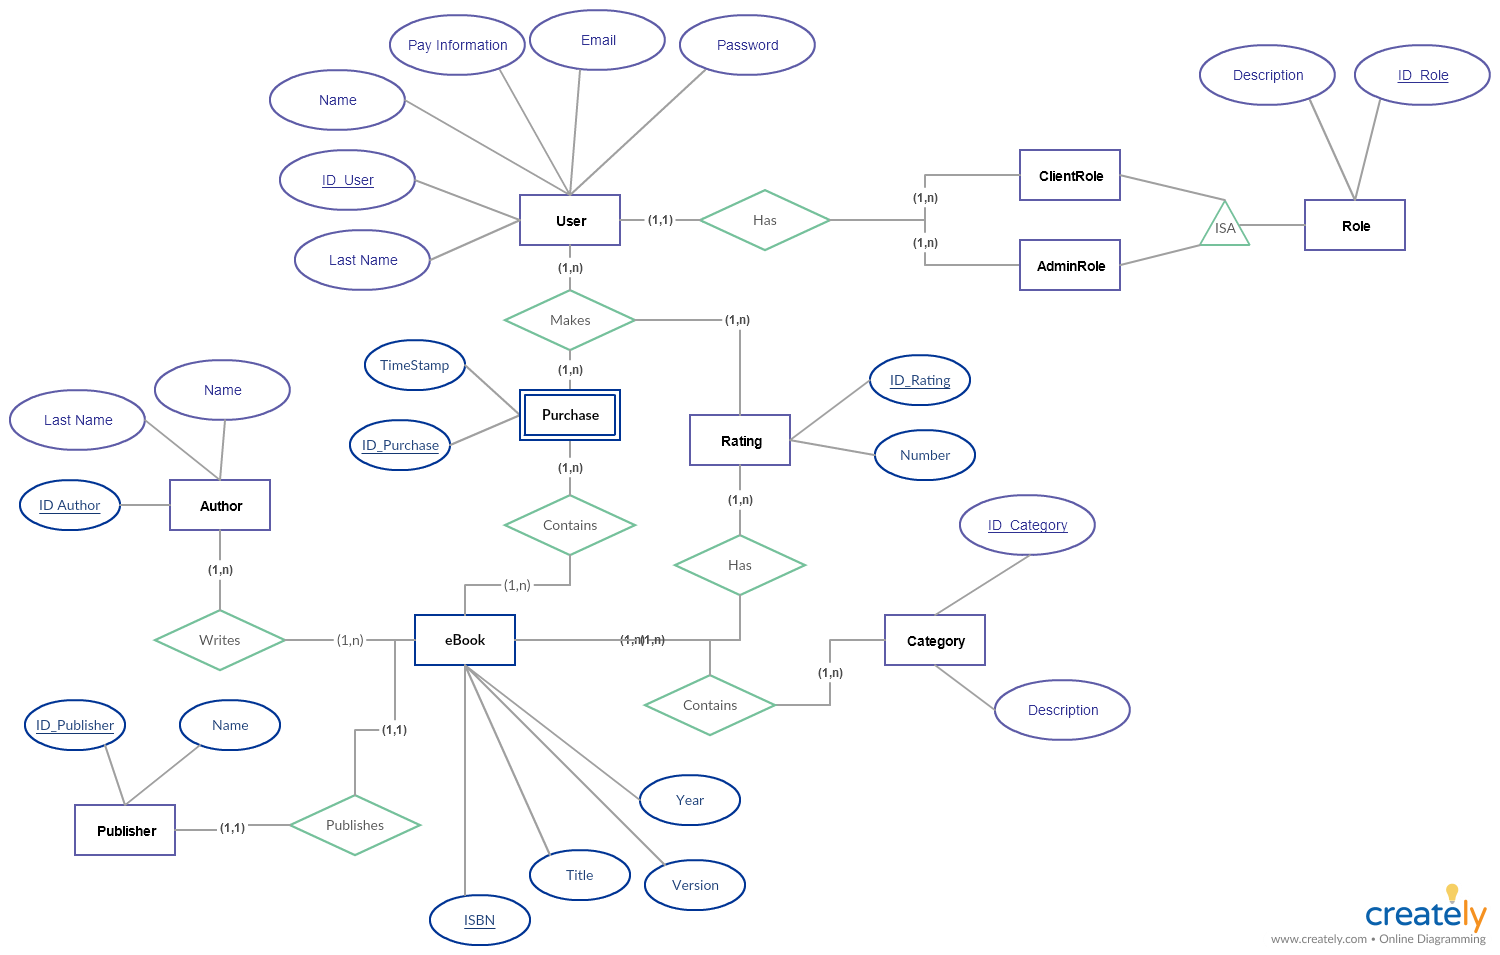
\includegraphics[width=\paperwidth]{ER_graph.png}}
\end{center}
\section{WebOwl}
\begin{center}
  \makebox[\textwidth]{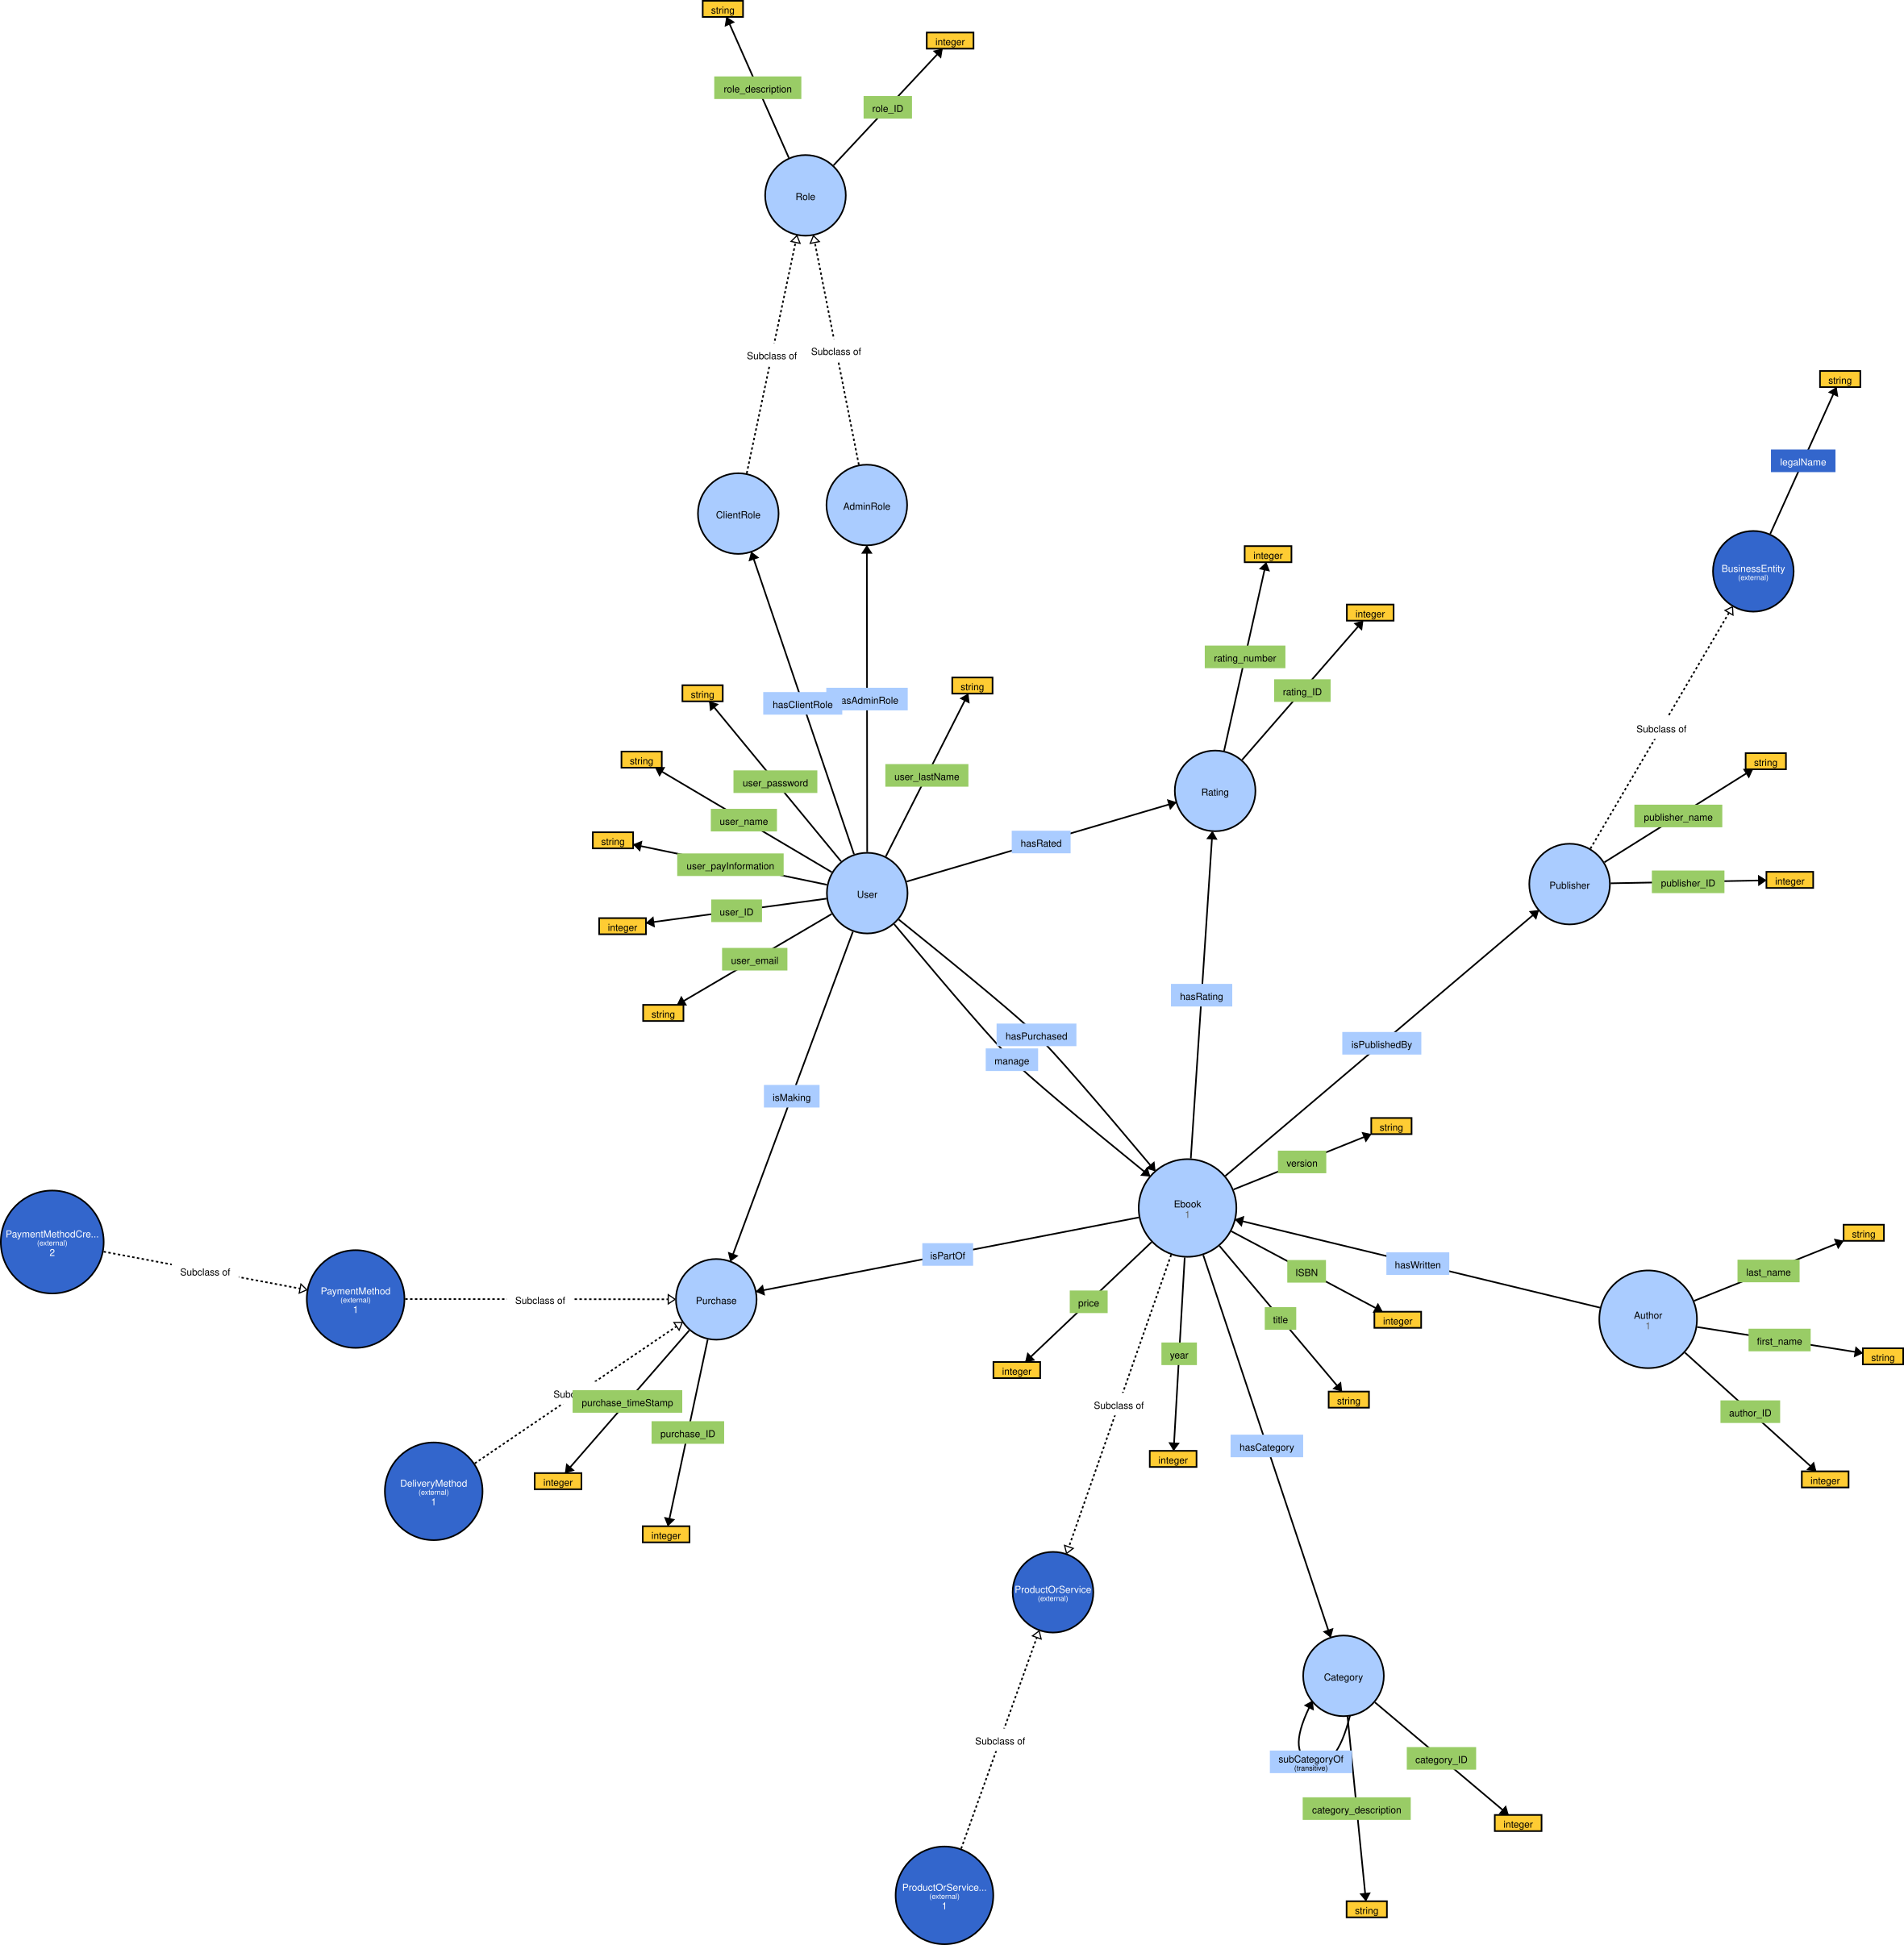
\includegraphics[width=\paperwidth]{webOwl.png}}
\end{center}

\end{document}
